\documentclass[landscape, 8pt, a4paper, oneside, twocolumn]{article}

\usepackage[utf8]{inputenc}
\usepackage[english]{babel}
\usepackage[T2A]{fontenc}

\usepackage{color}
\usepackage{fancyhdr}
\usepackage{geometry}
\usepackage{lastpage}
\usepackage{listings}
\usepackage{minted}
\usepackage{titletoc}
\usepackage{verbatim}
\usepackage{amsmath}
\usepackage{graphicx}
\usepackage{pdfpages}
\usepackage{tikz}

\geometry{
		margin=2cm,
		left=1cm,
		right=1cm
}

\pagestyle{fancy}
\lhead{Moscow SU Red Panda}
\rhead{\thepage\ of \pageref{LastPage}}
\fancyfoot{}
\dottedcontents{section}[3.0em]{\bfseries}{2.5em}{0pc}
\dottedcontents{subsection}[4.5em]{}{3.5em}{0.75pc}
\setlength{\columnseprule}{0.4pt}
\setlength\parindent{0pt}
\setminted{breaklines, tabsize=4}

\newcommand{\addalgorithm}[2]{
	\subsection{#1}
	\inputminted{C++}{#2}
}

\newcommand{\addtex}[2]{
	\subsection{#1}
	\input{#2}
}

\title{Team Notebook of Moscow SU Red Panda}
\date{Compiled on \today}

\begin{document}
	\section{Environment}
	%TODO middle mouse button
	\addtex{Linux}{tex/linux.tex}
	\addtex{.vimrc}{tex/vimrc.tex}
	\addalgorithm{C++ template}{algo/template.cpp}
	\newpage
	\tableofcontents
	\addtex{Table}{tex/table.tex}
	\newpage
	\section{Math}
	\addtex{Integrals}{tex/integrals.tex}
	\section{Tricks}
	\addalgorithm{GCC}{algo/gcc.cpp}
	\addalgorithm{Mult}{algo/mult.cpp}
	\section{Popular Algos}
	\addalgorithm{Hungary}{algo/hungary.cpp}
	\addalgorithm{CHT}{algo/chtVlad.cpp}
	\section{Geometry}
	\addalgorithm{HPI}{algo/hpint.cpp}
	\addtex{Radical Axis}{tex/radax.tex}
	\addalgorithm{Hull3d}{algo/lewin3d.cpp}
	\addtex{Another Hull3d}{tex/hull3d2.tex}
	\addalgorithm{Simplex}{algo/simplex.cpp}
	\section{Strings}
	\addalgorithm{Eertree}{algo/palin.cpp}
	\addalgorithm{SufArray}{algo/sufarray.cpp}
	\addalgorithm{SufAuto}{algo/sufauto.cpp}
	\addalgorithm{SufTree}{algo/suftree.cpp}
	\addalgorithm{Tandem}{algo/tandem.cpp}
	\section{Number Theory}
	\addtex{Numbers}{tex/nt.tex}
	\addalgorithm{Prefix Inverse O(n)}{algo/revOn.cpp}
	\addalgorithm{Gonchar Fedor}{algo/fedor.cpp}
	\addtex{Primes < n}{tex/primes.tex}
	\section{Numerical}
	\addtex{Runge-Kutta}{tex/rk.tex}
	\addalgorithm{Gaussian Quadrature}{algo/int.cpp}
	\section{Other}
	\addalgorithm{Walsh-Hadamard}{algo/Walsh-Hadamard.cpp}
	\addalgorithm{Global MinCut}{algo/wagner.cpp}
	\addtex{Matroids}{tex/matroids.tex}
	\addtex{Min Mean Cycle}{tex/meancycle.tex}
	\addalgorithm{General Matching}{algo/match.cpp}
	\addtex{Java}{tex/java.tex}
	\addalgorithm{Link-Cut Tree}{algo/linkcut.cpp}
	\subsection{Minimum directed spanning tree}
Given a weighted directed graph with a fixed root vertex $r$, find a set of edges with minimum total weight that makes all vertices reachable from $r$.

\subsubsection*{$O(nm)$ solution}
\begin{enumerate}
\item For each vertex $v \ne r$, consider the weights of all incoming edges: $w_1, w_2, \ldots, w_k$. Subtract $\min(w_1, w_2, \ldots, w_k)$ from each of $w_1, w_2, \ldots, w_k$. We'll denote this operation as \textit{nullifying} vertex $v$.
\item If every node is \textit{zero-reachable} from $r$ (reachable by zero-weight edges), break.
\item Compress SCCs consisting of zero-weight edges (or just compress any zero-weight cycle) and repeat.
\end{enumerate}

\subsubsection*{$O(m \log^\alpha n)$ solution}
\begin{enumerate}
\item Pick any vertex $v$ that is not zero-reachable from $r$. Let $v_0 = v$.
\item For each $i$, nullify $v_i$ and let $v_{i+1}$ be any vertex such that edge $(v_{i+1}, v_{i})$ has weight 0.
\item If at some point $v_i$ is zero-reachable from $r$, return to step 1 and pick another $v$ (if any).
\item If $v_i = v_j$ for $j < i$, we have found a zero-weight cycle. Compress this cycle into a new vertex $u$. \newline Set $v_j \gets u$, set $i \gets j$, and go to step 2.
\end{enumerate}
How to perform these steps efficiently?
\begin{itemize}
\item For each vertex $v$, store all edges incoming into $v$ in a data structure (DS) that allows extracting the smallest element, changing all elements of DS by the same constant, and merging two DS into a single one. Options:
 \begin{itemize}
  \item \texttt{std::set} with a global shift (insert elements from small to large $\rightarrow$ merge in $O(\log^2 n)$ amortized)
  \item \textit{treap} with implicit keys, minimum on subtrees and lazy propagation ($O(\log n)$)
  \item leftist heap, pairing heap, randomized meldable heap... ($O(\log n)$)
 \end{itemize}
\item Keep all vertices in a DSU (disjoint set union). Moving from $v_i$ to $v_{i+1}$, unite their sets in DSU. Now $v$ is zero-reachable from $r$ iff it is in the same set.
\end{itemize}
\subsection{Dominator tree}
Given a directed graph with a fixed root vertex $r$, vertex $u$ \textit{dominates} vertex $v$ if every path from $r$ to $v$ contains~$u$. Build a tree rooted at $r$ such that $u$ dominates $v$ in the graph iff $u$ is an ancestor of $v$ in the tree.
\newline \newline
Vertex $u = idom(v)$ is an \textit{immediate dominator} of vertex $v$ iff $u$ is the parent of $v$ in the dominator tree.
\subsubsection*{For a directed acyclic graph}
\begin{enumerate}
\item For each vertex $v$ in order of topological sorting of the graph, we will find $idom(v)$.
\item Consider all edges incoming into $v$: $(u_1, v)$, $(u_2, v)$, $\ldots$, $(u_k, v)$.
\item Every dominator of $v$ must be dominating $u_1, u_2, \ldots, u_k$ at the same time.
\item $idom(v)$ is the least common ancestor (LCA) of $u_1, u_2, \ldots, u_k$ in the dominator tree.
\item LCA of two vertices can be found with binary lifting in $O(\log n)$. Jumps of sizes $2^k$ from $v$ must be calculated after finding $idom(v)$. The overall complexity is $O(m \log n)$.
\end{enumerate}

\subsubsection*{For a general directed graph}
\begin{enumerate}
\item Perform a depth-first search (DFS) on the graph. Renumerate the vertices in order of first visit.
\item Graph edges can be directed top-to-bottom, bottom-to-top, right-to-left, but not left-to-right in the DFS tree.
\item \textit{Semidominator} $sdom(v)$ of vertex $v$ is the smallest vertex $u$ such that there exists a path $u = v_0, v_1, \ldots, v_k = v$ such that $v_i > v$ for $1 \le i < k$.
\item $sdom(v)$ and $idom(v)$ are ancestors of $v$ in the DFS tree.
\item Consider the following graph: the edges of the DFS tree plus edges $(sdom(v), v)$ for all $v \ne r$. The dominator tree for this graph is the same as for the original graph. But this graph is acyclic, and we already know how to build the dominator tree for acyclic graphs quickly.
\end{enumerate}
Observations required for finding semidominators:
\begin{enumerate}
\item Consider all edges incoming into vertex $v$: $(u_1, v)$, $(u_2, v)$, $\ldots$, $(u_k, v)$.
\item If $u_i$ is an ancestor of $v$ in the DFS tree, $u_i$ is a candidate for $sdom(v)$.
\item Otherwise, consider all vertices $w$ that are ancestors of $u$ but not of $v$: $sdom(w)$ is a candidate for $sdom(v)$.
\item $sdom(v)$ is the smallest numbered vertex out of all candidates.
\end{enumerate}
The actual algorithm for finding semidominators in $O(m \log n)$:
\begin{enumerate}
\item Place all vertices in a disjoint set union (DSU). Every set in the DSU is a rooted tree. For each vertex $v$, store the minimum of $sdom$ on the path from $v$ to its parent in the DSU set.
\item Process vertices in decreasing order. After processing vertex $v$, link it to its DFS tree parent in the DSU. Note that rank heuristic can not be applied, but just path compression is enough for $O(\log n)$ per query.
\item When processing vertex $v$, for each edge $(u_i, v)$ such that $u_i$ is not an ancestor of $v$, compress the path from $u_i$ to its root in the DSU. Now the minimum of $sdom$ we are storing for $u_i$ is the candidate for $sdom(v)$.
\end{enumerate}

	\addtex{Tree hash}{tex/tree_hash.tex}
	\addalgorithm{Weighted Matching}{algo/weightedmatching.cpp}
	\addalgorithm{Berlekamp-Massey}{algo/bm.cpp}
	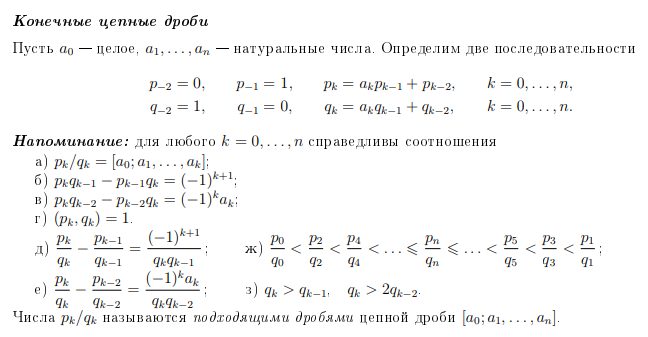
\includegraphics[scale=0.75,angle=90]{pics/confrac.png}
	\subsection{Integrals}
	\onecolumn
	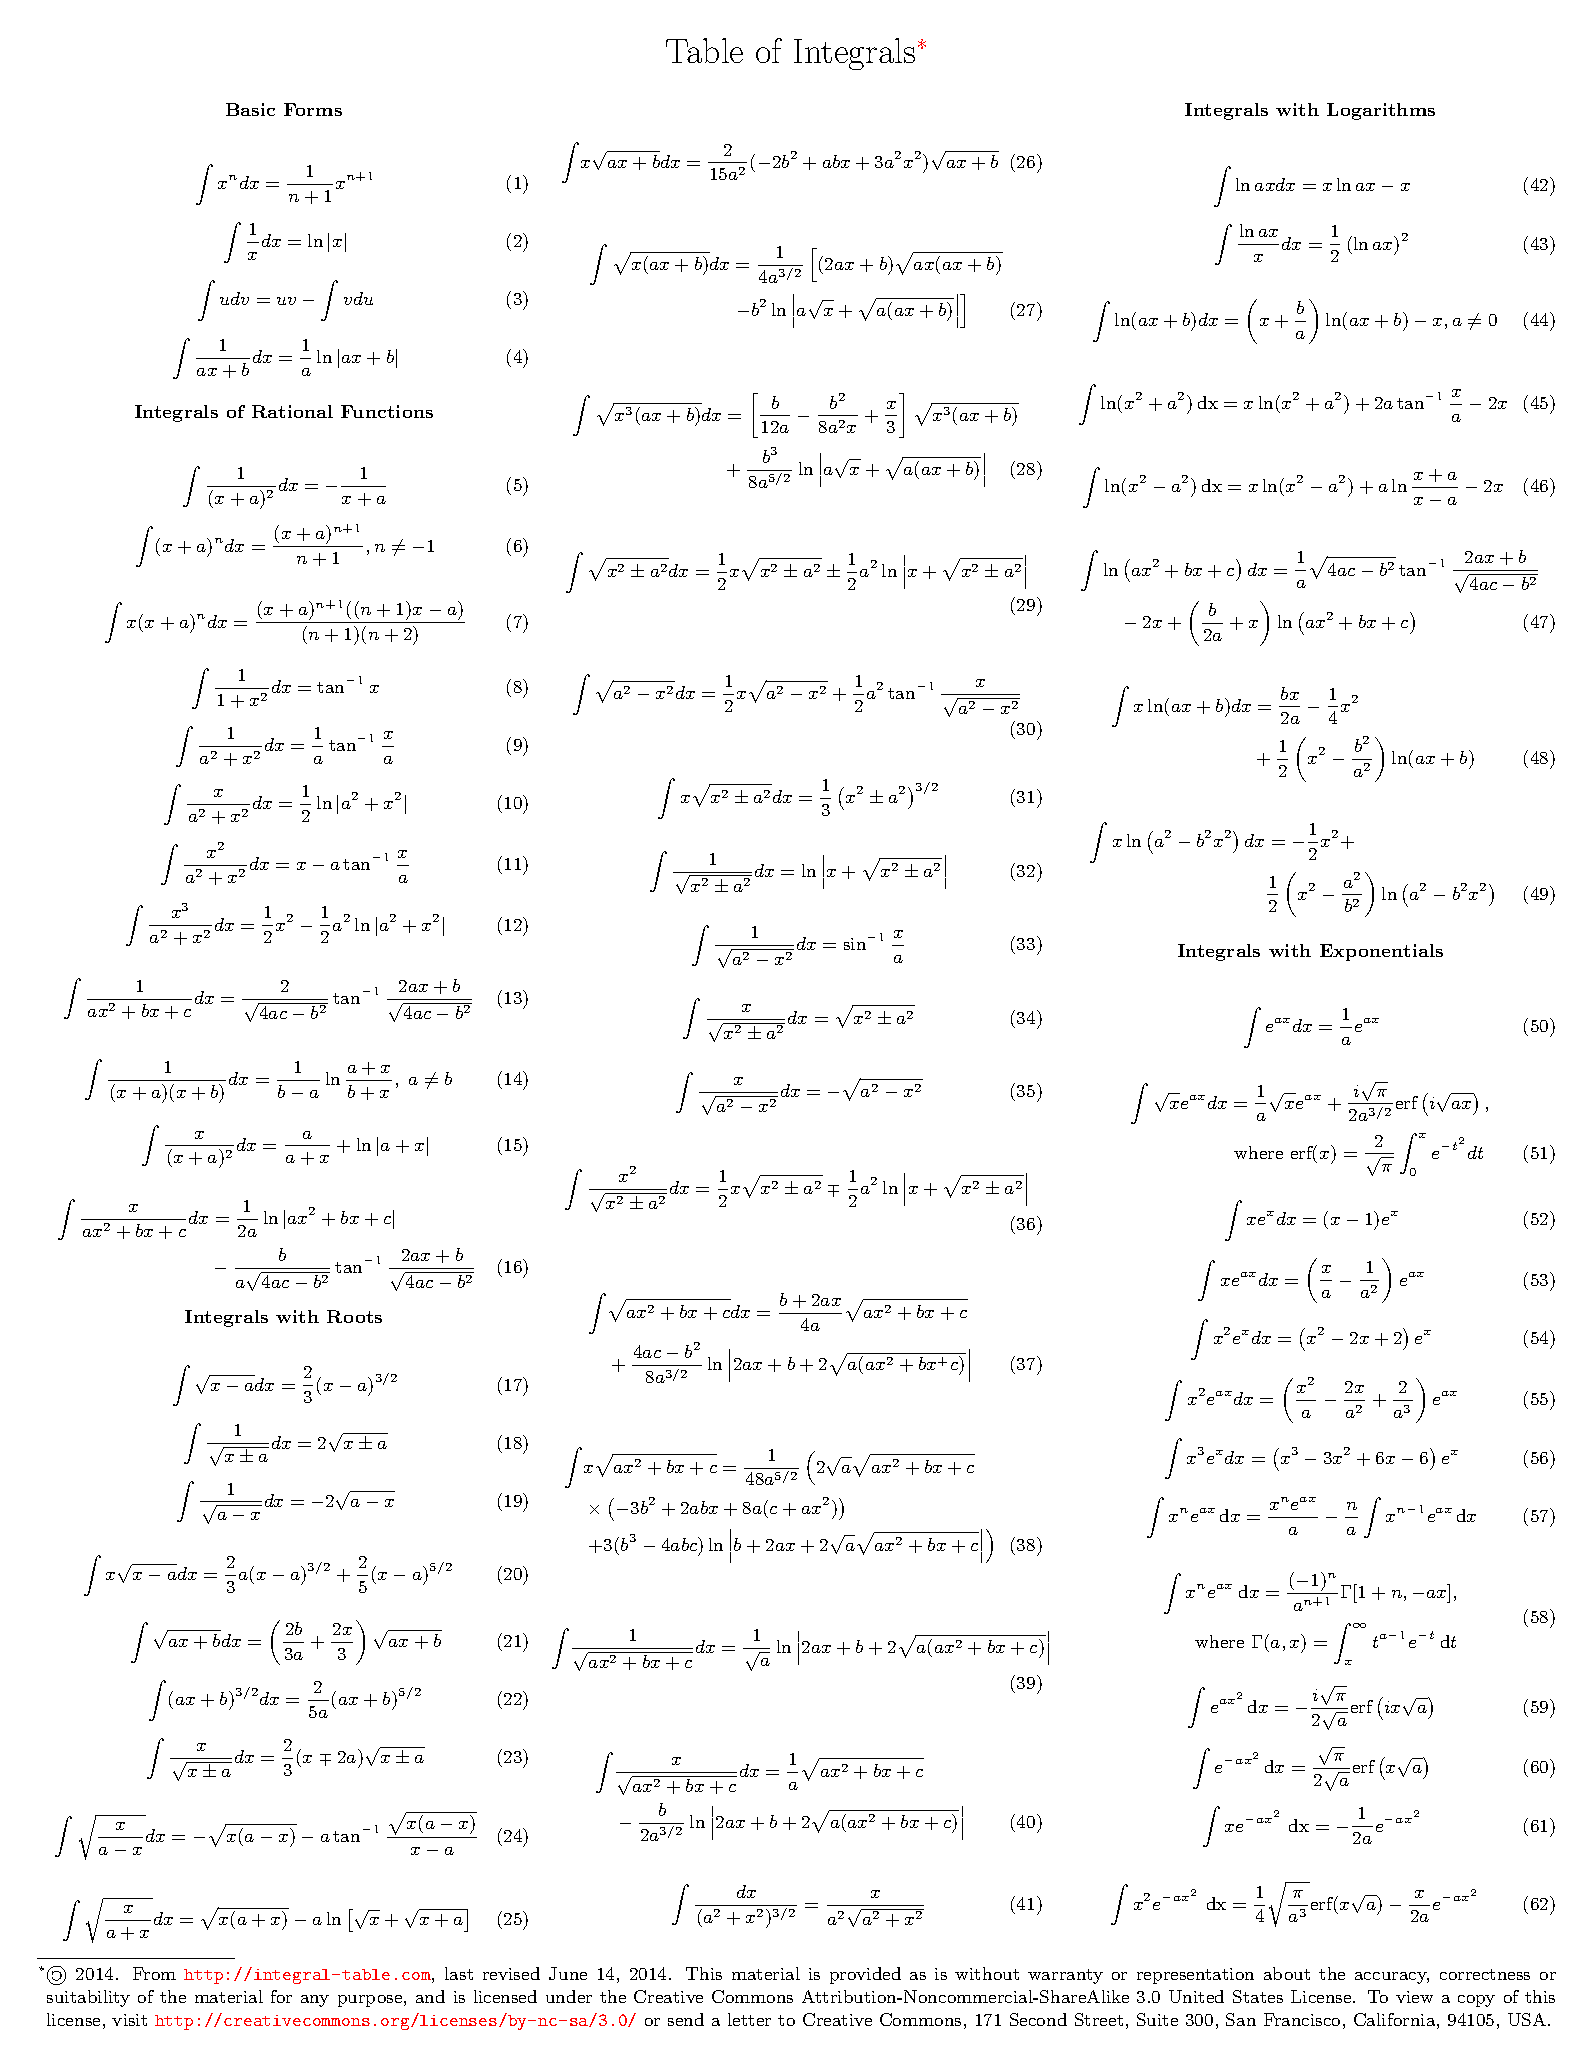
\includepdf[angle=90,scale=0.9,pages=-,pagecommand={\pagestyle{fancy}}]{pdf/integralTable.pdf}
	\addtex{Hexagon}{tex/hexagon.tex}
	\newpage
	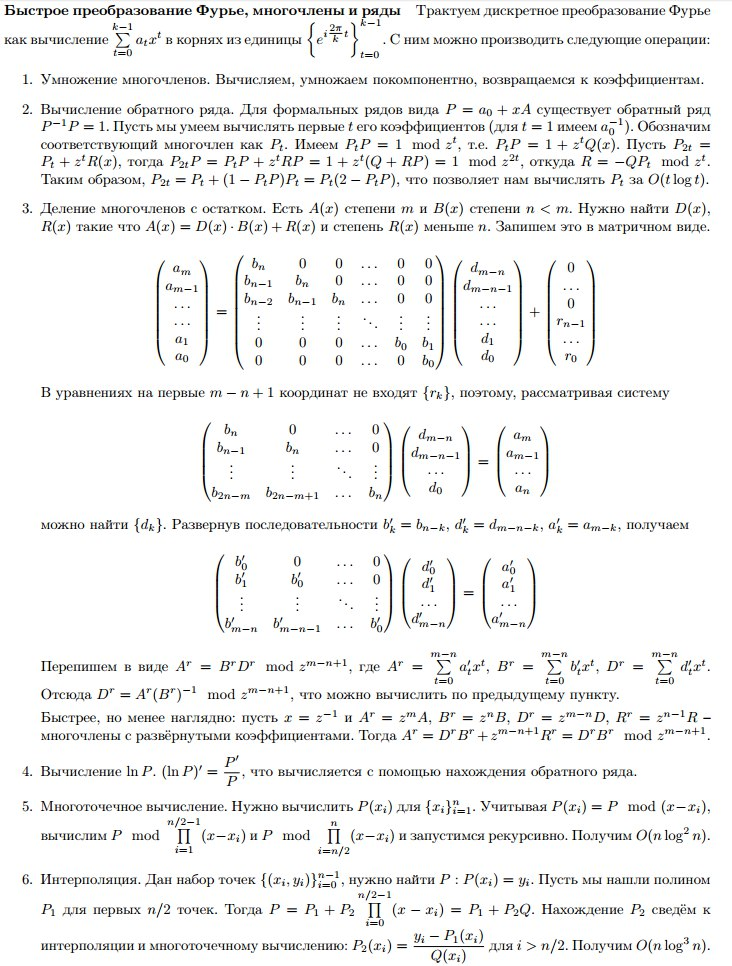
\includegraphics[scale=0.6,angle=90]{pics/adamant.jpg}

\end{document}
